\documentclass[compress]{beamer}        % [compress] (written before {beamer} <=> navigation bar one line, all subsections in 1 line instead of 2

% Setup appearance:
\usetheme{CambridgeUS}
%	AnnArbor | Antibes | Bergen |
%	Berkeley | Berlin | Boadilla |
%	boxes | CambridgeUS | Copenhagen |
%	Darmstadt | default | Dresden |
%	Frankfurt | Goettingen |Hannover |
%	Ilmenau | JuanLesPins | Luebeck |
%	Madrid | Malmoe | Marburg |
%	Montpellier | PaloAlto | Pittsburgh |
%	Rochester | Singapore | Szeged |
%	Warsaw
%

\useoutertheme[footline=authorinstitute,subsection=false]{miniframes}
\usecolortheme{whale}

%	albatross | beaver | beetle |
%	crane | default | dolphin |
%	dove | fly | lily | orchid |
%	rose |seagull | seahorse |
%	sidebartab | structure |
%	whale | wolverine


\setbeamertemplate{footline}
{
  \hbox{%
  \begin{beamercolorbox}[wd=.25\paperwidth,ht=2.25ex,dp=1ex,center]{title in head/foot}%
    \usebeamerfont{date in head/foot}\insertshortauthor
  \end{beamercolorbox}%
  \begin{beamercolorbox}[wd=.5\paperwidth,ht=2.25ex,dp=1ex,center]{date in head/foot}%
    \usebeamerfont{title in head/foot}\insertshortinstitute
  \end{beamercolorbox}%
  \begin{beamercolorbox}[wd=.25\paperwidth,ht=2.25ex,dp=1ex,center]{title in head/foot}%
    \usebeamerfont{date in head/foot}
    \insertframenumber{} / \inserttotalframenumber
    %\insertframenumber{} / \insertpresentationendpage
  \end{beamercolorbox}}%
  \vskip0pt%
}

%\setbeamercolor{titlelike}{parent=structure}
%\setbeamercolor{structure}{fg=beamer@blendedblue}
%% \useinnertheme{rounded}
%\setbeamerfont{block title}{size={}}
%\usefonttheme[onlylarge]{structurebold}   % title and words in the table of contents bold
%\setbeamerfont*{frametitle}{size=\normalsize,series=\bfseries}
\setbeamertemplate{navigation symbols}{}
\setbeamercolor{frametitle}{parent=boxes, bg=white}
{ % only on titlepage


\usepackage{times}
\usepackage{amsmath,amssymb,amsthm}
\usepackage{color}
\usepackage{changepage}
\usepackage{multirow}
\usepackage[absolute,overlay]{textpos}
\usepackage{enumerate}
%\usepackage{pgfpages}
\usepackage[all]{xy}
\usepackage{textcomp}
\usepackage{etex}
\usepackage{tikz}
\usetikzlibrary{shapes}
%\usepackage{handoutWithNotes}
%\pgfpagesuselayout{4 on 1}[border shrink=1mm]




\definecolor{camblue}{RGB}{26,26,89}
\definecolor{Rblue}{RGB}{0,255,255}
\definecolor{Rdarkblue}{RGB}{0,0,255}
\definecolor{Rgreen}{RGB}{0,205,0}
\definecolor{green2}{RGB}{51,204,51}
\newcommand{\tcb}{\textcolor{beamer@blendedblue}}
\newcommand{\tcbb}{\textcolor{camblue}}
\newcommand{\tcr}{\textcolor{red}}
\newcommand{\tcg}{\textcolor{gray}}
\newcommand{\tcgr}{\textcolor{green2}}
\newcommand{\tcblk}{\textcolor{black}}
\newcommand{\tcRg}{\textcolor{Rgreen}}
\newcommand{\tcRdb}{\textcolor{Rdarkblue}}
\newcommand{\tcRb}{\textcolor{Rblue}}
\newcommand{\tcw}{\textcolor{white}}
\newcommand{\m}{\phantom{-}}
\newcommand{\bp}{\tcbb{$\bullet$}\:}


\title{{\huge Statistics for Computing\\[0.1cm]MA4413}}
\author[Kevin Burke]{{\bf\\[0.5cm]{\huge Lecture 4}\\[0.2cm]\emph{Conditional Probability, Law of Total Probability\\and Bayes' Rule}\\[1.4cm]Kevin Burke}\\[0.3cm]\tcb{kevin.burke@ul.ie}}

\institute[University of Limerick, Maths \& Stats Dept]{}
\date{}

%\TPGrid[5mm,5mm]{1}{1}

\begin{document}


\begin{frame}[t]
\titlepage
\end{frame}


\section{Conditional Probability}
\subsection{Conditional Probability}
\begin{frame}{\bf \tcb{Conditional Probability}}
In the previous lecture we encountered {\bf conditional probability}, i.e.,\\[0.1cm]
\begin{align*}
\Pr(A\,|\,B)\\[-0.3cm]
\end{align*}
which represents an \emph{updated} probability of $A$ given the \emph{information} that $B$ has occurred.\\[0.8cm]
Good decisions should be based on using the information at hand.\\[0.8cm]
\end{frame}


\subsection{Conditional Probability}
\begin{frame}{\bf \tcb{Conditional Probability}}
Let's assume that we have some idea about the probability of a bug in some software, for example, $\Pr(\text{bug}) = 0.1$.\\[0.6cm]
We are then given \emph{new information}: the code was written by an inexperienced programmer.\\[0.6cm]
How would we \emph{update} our \emph{prior} probability of $\Pr(\text{bug}) = 0.1$?
\begin{align*}
\Pr(\text{bug}\,|\,\text{inexperienced}) &< 0.1?\\[0.2cm]
\Pr(\text{bug}\,|\,\text{inexperienced}) &= 0.1?\\[0.2cm]
\Pr(\text{bug}\,|\,\text{inexperienced}) &> 0.1?
\end{align*}
\end{frame}


\subsection{Conditional Probability}
\begin{frame}{\bf \tcb{Conditional Probability}}

It should be quite clear that ``bug in software'' and ``inexperienced programmer'' are \emph{dependent events}.\\[0.3cm]
Furthermore, it is reasonable to expect $\Pr(\text{bug}\,|\,\text{inexperienced}) > 0.1$.\\[0.6cm]
\hrule\vspace{0.6cm}

What if we had been told that the programmer has brown hair instead?\\[0.3cm]
We might imagine that programming ability and hair colour are \emph{independent events} so that $\Pr(\text{bug}\,|\,\text{brown hair}) = \Pr(\text{bug}) = 0.1$.\\[0.6cm]
\hrule\vspace{0.6cm}

Can you think of an event that might lead to  $\Pr(\text{bug}\,|\,\text{event}) < 0.1$?
\end{frame}


\subsection{Conditional Probability Formula}
\begin{frame}{\bf \tcb{Conditional Probability Formula}}
Recall from the previous lecture (multiplication rule) that
\begin{align*}
\Pr(B) \Pr(A \,|\, B) = \Pr(A \cap B).\\[0.4cm]
\end{align*}

Dividing both sides by $\Pr(B)$ gives us a formula for calculating {\bf conditional probability}:\\[-0.2cm]
\begin{align*}
\boxed{\Pr(A \,|\, B) = \frac{\Pr(A \cap B)}{\Pr(B)}}.
\end{align*}

\end{frame}


\subsection{Conditional Probability Formula}
\begin{frame}{\bf \tcb{Conditional Probability Formula}}

We get an expression for $\Pr(B \,|\, A)$ by swapping the letters around:\\[0.2cm]
\begin{align*}
\Pr(B \,|\, A) = \frac{\Pr(B \cap A)}{\Pr(A)} = \frac{\Pr(A \cap B)}{\Pr(A)}\\
\end{align*}
since $\Pr(B \cap A) = \Pr(A \cap B)$.\\[1.6cm]
Note that $\Pr(A \,|\, B)$ and $\Pr(B \,|\, A)$ are \emph{not} the same thing.

\end{frame}


\subsection{Example: Flipping a Coin and Rolling a Die}
\begin{frame}{\bf \tcb{Example: Flipping a Coin and Rolling a Die}}
In the previous lecture we dealt with the experiment of flipping a coin and rolling a die.\\[0.3cm]
We had the events\\[0.0cm]
\begin{itemize}\itemsep0.2cm
\item $A =$ ``head \& even number''.
\item $B =$ ``head \& any number'' $=$ ``the coin shows a head''.
\item $C =$ ``any face \& a five'' $=$ ``the die shows a five''.\\[0.3cm]
\end{itemize}

We calculated\\[0.0cm]
\begin{itemize}\itemsep0.2cm
\item $\Pr(A) = \tfrac{1}{4}$, $\Pr(B) = \tfrac{1}{2}$ and $\Pr(C) = \tfrac{1}{6}$.
\item $\Pr(A \cap B) = \tfrac{1}{4}$, $\Pr(A \cap C) = 0$ and $\Pr(B \cap C) = \tfrac{1}{12}$.\\[0.3cm]
\end{itemize}

We also worked out which events were independent and dependent but now, using the formula for \emph{conditional probability}, we can go further.

\end{frame}


\subsection{Example: Flipping a Coin and Rolling a Die}
\begin{frame}{\bf \tcb{Example: Flipping a Coin and Rolling a Die}}
Consider
\begin{align*}
\Pr(A\,|\,B) = \frac{\Pr(A \cap B)}{\Pr(B)} =\,\,\, \frac{\tfrac{1}{4}}{\tfrac{1}{2}} \,\,\,=\,\,\, \frac{2}{1} \times \frac{1}{4} \,\,\,=\,\,\, \frac{2}{4} \,\,\,=\,\,\, \frac{1}{2}.\\[-0.4cm]
\end{align*}

Thus,\\[0.1cm]
\begin{itemize}\itemsep0.4cm
\item $\Pr(A) = \Pr(\text{``head \& even''}) = \tfrac{1}{4} = 0.25$.
\item $\Pr(A\,|\,B) = \Pr(\text{``head \& even''}\,|\,\text{``coin shows head''}) = \tfrac{1}{2} = 0.5$.\\[0.8cm]
\end{itemize}

This result makes intuitive sense: since we now know that the coin shows a head, we are more sure about the result being ``head \& even''.\\[0.4cm]
We \emph{update} the \emph{prior} probability using the current \emph{information}.

\end{frame}



\subsection{Example: Flipping a Coin and Rolling a Die}
\begin{frame}{\bf \tcb{Example: Flipping a Coin and Rolling a Die}}
A more detailed explanation of the previous result:\\[1.1cm]

Without any information, there are twelve possible outcomes $\{H1,H2,H3,H4,H5,H6,T1,T2,T3,T4,T5,T6\}$.\\[0.3cm]
Three of these (i.e., 25\%) fall into the category ``head \& even''.\\[1cm]

Given the information that the coin shows a head, there are now only six possible outcomes $\{H1,H2,H3,H4,H5,H6\}$.\\[0.3cm]
Three of these (i.e., 50\%) fall into the category ``head \& even''.
\end{frame}


\subsection{Example: Flipping a Coin and Rolling a Die}
\begin{frame}{\bf \tcb{Example: Flipping a Coin and Rolling a Die}}
Let's now consider
\begin{align*}
\Pr(A\,|\,C) = \frac{\Pr(A \cap C)}{\Pr(C)} =\,\,\, \frac{0}{\tfrac{1}{6}} \,\,\,=\,\,\, \frac{6}{1} \times 0 \,\,\,=\,\,\, 0.\\[-0.4cm]
\end{align*}

Thus,\\[0.1cm]
\begin{itemize}\itemsep0.4cm
\item $\Pr(A) = \Pr(\text{``head \& even''}) = \tfrac{1}{4} = 0.25$.
\item $\Pr(A\,|\,C) = \Pr(\text{``head \& even''}\,|\,\text{``dies shows a five''}) = 0$.\\[0.8cm]
\end{itemize}

Given the information that the die shows a five, we know that the result cannot be ``head \& even'' $\Rightarrow$ our \emph{updated probability} is $\Pr(A\,|\,C) = 0$.

\end{frame}


\subsection{Question 1}
\begin{frame}{\bf \tcb{Question 1}}

Continue with the previous example of flipping a coin and rolling a die.\\[0.5cm]

\begin{enumerate}[a)]\itemsep0.4cm
\item Calculate $\Pr(B\,|\,A)$, $\Pr(C\,|\,A)$, $\Pr(B\,|\,C)$ and $\Pr(C\,|\,B)$.
\item Compare the above \emph{updated} probabilities with the relevant \emph{prior} probabilities. Give a brief explanation of the results.
\item Which events are independent?
\item Which events are mutually exclusive?
\end{enumerate}

\end{frame}


\subsection{Question 2}
\begin{frame}{\bf \tcb{Question 2 (questions on next slide)}}
A software company examined blocks of code written by its employees. Each block of code was tested for bugs and, in addition, the skill level of the employee was also recorded. See table below.
\begin{center}
\begin{tabular}{|cc|ccc|c|}
\hline
&&&&&\\[-0.4cm]
    && \multicolumn{3}{|c|}{Skill Level} &  \\
    && High & Average & Low & Total \\
\hline
&&&&&\\[-0.4cm]
Bug in   & No    &  140 &   600  & 100 & 840 \\
Code & Yes   &    5 &    70  &  40 & 115 \\
\hline
&&&&&\\[-0.4cm]
&Total &  145 &   670  & 140 & 955 \\
\hline
\end{tabular}
\end{center}

We will let $B =$ ``bug'' and, hence, $B^c =$ ``no bug''.\\[0.2cm]
Also let $S_H = $ ``skill: high'', $S_A = $ ``skill: average'' and $S_L =$ ``skill: low''.\\[0.5cm]

Note that $S_H \cap B^c$ contains 140 cases, $S_H \cap B$ contains 5 cases, $H$ contains 145 cases etc.

\end{frame}



\subsection{Question 2}
\begin{frame}{\bf \tcb{Question 2}}
Note: Use the appropriate probability notation.\\[0.3cm]
\begin{enumerate}[a)]\itemsep0.3cm
\item Calculate the probability that the programmer has: (i) high skill, \\(ii) average skill and (iii) low skill.
\item Calculate the probability of a bug.
\item Calculate the probability of a bug \emph{given that} the code was written by a programmer with: (i) high skill, (ii) average skill and (iii) low skill.
\item Comment on the above conditional (i.e., updated) probabilities compared with $\Pr(B)$ calculated in part (b). Is the presence of bugs independent of the skill level?
\item Show that $\Pr(S_A\,|\,B) > \Pr(S_L\,|\,B)$. Explain the reason for this.
\end{enumerate}


\end{frame}








\section{Law of Total Probability}
\subsection{Law of Total Probability}
\begin{frame}{\bf \tcb{Law of Total Probability}}

\begin{center}
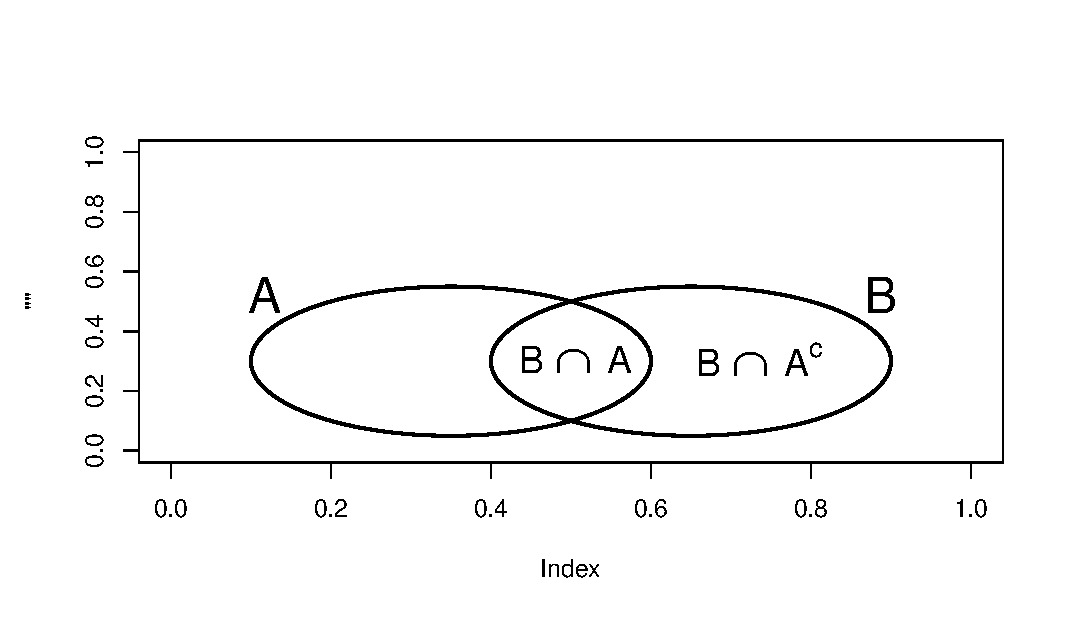
\includegraphics[width=0.6\textwidth, trim = 3.5cm 3cm 2.5cm 4.3cm, clip]{totalprob}
\end{center}

From the above we can see that
\begin{align*}
\Pr(B) = \Pr(B \cap A) + \Pr(B \cap A^c).\\[-0.3cm]
\end{align*}
Also $\Pr(B \cap A) = \Pr(A) \Pr(B \,|\, A)$ and $\Pr(B \cap A^c) = \Pr(A^c) \Pr(B \,|\, A^c)$
using the \emph{multiplication rule}.\\[-0.2cm]

\begin{align*}
\Rightarrow \boxed{\Pr(B) = \Pr(A) \Pr(B \,|\, A) + \Pr(A^c) \Pr(B \,|\, A^c)}.
\end{align*}
This is the simplest example of the {\bf law of total probability}.

\end{frame}


\subsection{Law of Total Probability}
\begin{frame}{\bf \tcb{Law of Total Probability}}

\begin{center}
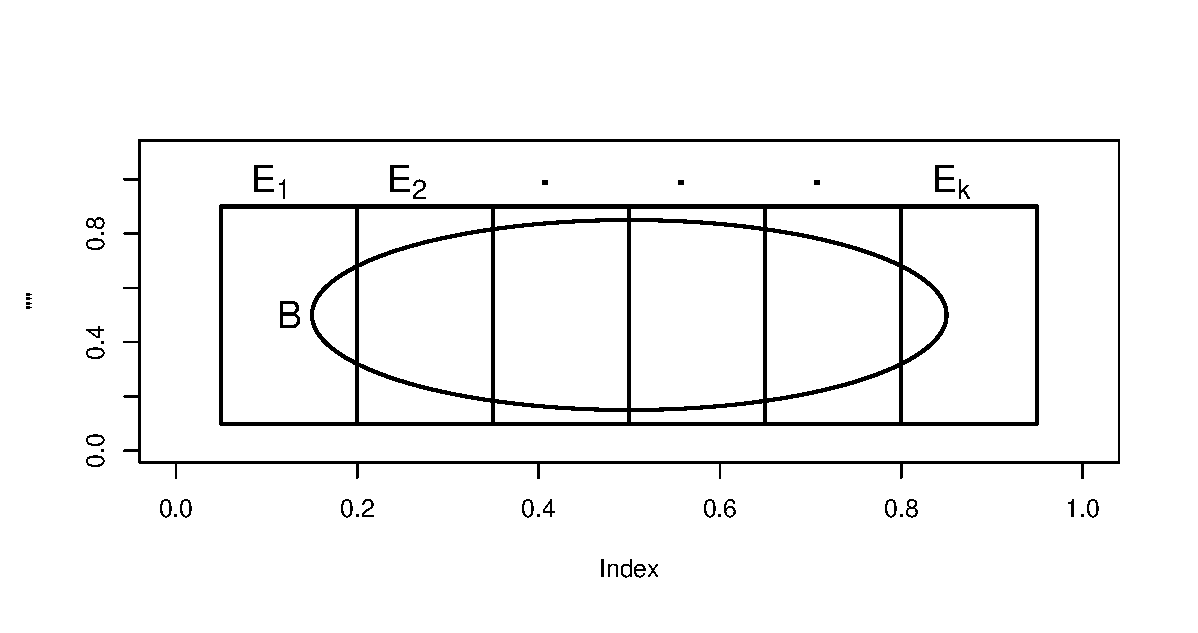
\includegraphics[width=0.8\textwidth, trim = 3.3cm 3cm 2.3cm 2.5cm, clip]{totalprob2}
\end{center}

If there are $k$ \emph{mutually exclusive} and \emph{exhaustive} events, $E_1,E_2,\ldots,E_k$, then the {\bf law of total probability} is\\[-0.7cm]

\begin{adjustwidth}{-0.25cm}{0.1cm}
\begin{tabular}{|c@{\,\,$=$\,\,}c@{\,\,$+$\,\,}c@{\,\,$+$\,\,}c@{\,$+$\,\,}c|}
\hline
\multicolumn{5}{|c|}{}\\[-0.4cm]
$\Pr(B)$ & $\Pr(B \cap E_1)$ & $\Pr(B \cap E_2)$ & $\cdots$ & $\Pr(B \cap E_k)$ \\[0.2cm]
         & $\Pr(E_1) \Pr(B \,|\, E_1)$ & $\Pr(E_2) \Pr(B \,|\, E_2)$ & $\cdots$ & $\Pr(E_k) \Pr(B \,|\, E_k)$\\[0.1cm]
\hline
\end{tabular}.
\end{adjustwidth}

\end{frame}



\subsection{Example: Internet Trolls}
\begin{frame}{\bf \tcb{Example: Internet Trolls}}

``Troll'' is the slang word used to describe an internet user who aims to irritate other users - often through the medium of comment posting.\\[0.6cm]

Let's assume that 10\% of internet users can be classed as trolls and that 99\% of their comments are irritating. Normal internet users (i.e., non-trolls) only post irritating comments 4\% of the time.\\[0.6cm]

If we let $T =$ ``the user is a troll'' and $I = $ ``the comment is irritating'' then from the information above we have:
\begin{align*}
\Pr(T) &= 0.1 & \Pr(I\,|\,T) & = 0.99 \\[0.2cm]
\Pr(T^c) &= 0.9 & \Pr(I\,|\,T^c) & = 0.04 \\
\end{align*}


\end{frame}


\subsection{Example: Internet Trolls}
\begin{frame}{\bf \tcb{Example: Internet Trolls}}

Using the \emph{law of total probability} we can work out the probability that an irritating comment is posted:

\begin{align*}
\Pr(I) = \Pr(I \cap T) + \Pr(I \cap T^c) &= \Pr(T) \Pr(I\,|\,T) + \Pr(T^c) \Pr(I\,|\,T^c) \\[0.2cm]
&= 0.1 (0.99) + 0.9(0.04) \\[0.2cm]
&= 0.099 + 0.036 \\[0.2cm]
&= 0.135.\\[-0.2cm]
\end{align*}

Thus, 13.5\% of comments are irritating.

\end{frame}



\subsection{Question 3}
\begin{frame}{\bf \tcb{Question 3}}

Return to the example used in Question 2.\\[0.3cm]
\begin{enumerate}[a)]\itemsep0.6cm
\item Calculate $\Pr(B)$ using the law of total probability and previously calculated values for $\Pr(B \cap S_H)$, $\Pr(B\cap S_A)$ and $\Pr(B\cap S_L)$.
\item Calculate $\Pr(S_H)$, $\Pr(S_A)$ and $\Pr(S_L)$ using similar means.\\[1.5cm]
\end{enumerate}
{\footnotesize(note: we previously calculated the \emph{total} probabilities directly from the table)}

\end{frame}



\section{Bayes' Rule}
\subsection{Bayes' Rule}
\begin{frame}{\bf \tcb{Bayes' Rule}}

{\bf Bayes' Rule} provides a method for assessing the likelihood of an event $E_1$ \emph{given} current information $B$.\\[0.5cm]

\emph{Bayes' Rule} is derived simply by combining the \emph{conditional probability} formula and the \emph{multiplication rule}:\\[0.1cm]
\begin{align*}
\boxed{\Pr(E_1 \,|\, B) = \frac{\Pr(E_1 \cap B)}{\Pr(B)} = \frac{\Pr(E_1) \Pr(B \,|\, E_1)}{\Pr(B)}},\\[-0.1cm]
\end{align*}

where, typically, $\Pr(B)$ is calculated using the \emph{law of total probability}, i.e., $\Pr(B) = \Pr(B \cap E_1) + \cdots + \Pr(B \cap E_k)$.

\end{frame}


\subsection{Example: Internet Troll Detection}
\begin{frame}{\bf \tcb{Example: Internet Troll Detection}}

We know from earlier that 13.5\% of all comments online are irritating, i.e., $\Pr(I) = 0.135.$\\[0.4cm]

We take a look at our blog and notice an irritating comment - was this the work of a troll?\\[0.4cm]

In other words, \emph{given that the message is irritating} what is the probability of a troll having posted it?\\[-0.2cm]

\begin{align*}
\Pr(T \,|\, I) =  \frac{\Pr(T) \Pr(I \,|\, T)}{\Pr(I)} &= \frac{0.1(0.99)}{0.135}\\[0.1cm]
&= \frac{0.099}{0.135}\\[0.1cm]
&\approx 0.73.
\end{align*}
There is a 73\% chance that this message was left by an internet troll.

\end{frame}

%
%\subsection{Example: Internet Troll Detection}
%\begin{frame}{\bf \tcb{Example: Internet Troll Detection}}
%
%What is the probability of a \emph{non-irritating} message was left by a troll?
%
%\begin{align*}
%\Pr(T \,|\, I^c) =  \frac{\Pr(T) \Pr(I^c \,|\, T)}{\Pr(I^c)} &= \frac{\Pr(T) [1 - \Pr(I \,|\, T)]}{1-\Pr(I)} \\[0.1cm]
%&= \frac{0.1(1-0.99)}{1-0.135}\\[0.1cm]
%&= \frac{0.1(0.01)}{0.865}\\[0.1cm]
%&= \frac{0.001}{0.865}\\[0.1cm]
%&\approx 0.0012.
%\end{align*}
%There is a 0.12\% (i.e., less than 1\%) chance that the message was left by an internet troll.
%
%\end{frame}



\subsection{Question 4}
\begin{frame}{\bf \tcb{Question 4}}

% phising, normal, advertisement emails

A manufacturer of laptops sources processors from three companies: $A_1$, $A_2$ and $A_3$. Specifically, 20\% of stock comes from $A_1$, $55\%$ comes from $A_2$ and the remainder comes from $A_3$. Assume that 10\% of $A_1$'s stock is defective, 4\% of $A_2$'s and 1\% of $A_3$'s.\\[0.3cm]

\begin{enumerate}[a)]\itemsep0.2cm
\item What is the probability that a defective processor is installed?
\item A customer comes back with a faulty laptop - we determine that the processor is the issue. Which company is most likely to have produced this processor?
\item What is the probability that a processor from $A_1$ works \emph{correctly}?
\item Given that the processor is working correctly, what is the probability it came from company $A_1$?
\item If \emph{all} stock came from $A_3$, what would $\Pr(D)$ be? What would $\Pr(A_3\,|\,D)$ be? What would $\Pr(A_1\,|\,D)$ be?
\end{enumerate}


\end{frame}








\end{document} 